\section{Composite Problems}
\begin{frame}{}
  \begin{center}
    {\bf Part III -- Composite Problems}
  \end{center}
\end{frame}

\begin{frame}[t]{Composite Problems}
  Until now, we could solve each problem with 1 algorithm.\bigskip

  But many interesting problems combine multiple algorithms!\bigskip

  A common combination is {\bf Binary Search + Solve smaller problem}:
  \begin{itemize}
    \item Binary Search + Geometry Problem;
    \item Binary Search + Graph Search;
    \item Binary Search + DP;
    \item Binary Search + Greedy;
    \item etc...
  \end{itemize}
\end{frame}

\subsection{Fatman}
\begin{frame}
  \frametitle{UVA 295 -- Fatman!}
  \begin{center}
    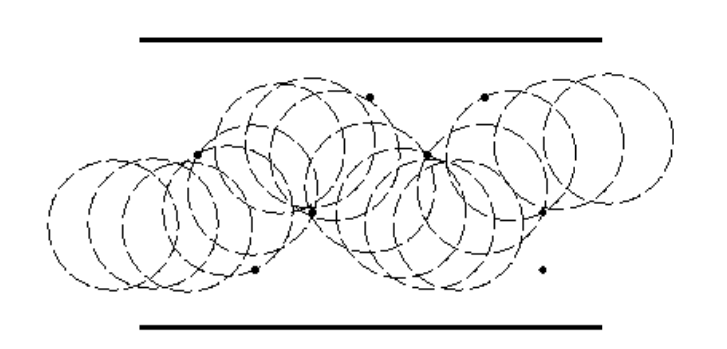
\includegraphics[width=0.5\textwidth]{img/fatman}
  \end{center}

  {\smaller
    \begin{block}{Problem Description}
      Find the {\bf maximum diameter D of the circle} that can pass the corridor.
      \begin{itemize}
      \item The corridor has length $L$ and width $W$;
      \item The corridor has $0 \leq N \leq 100$ obstacles, represented by $(x_i,y_i)$;
      \item Obstacles are {\bf points} with $0 \leq x_i \leq L, 0\leq y_i \leq W$;
      \end{itemize}
    \end{block}
  }
\end{frame}

\begin{frame}
  \frametitle{UVA 295 -- Fatman -- Breaking up the problem}
  \begin{center}
    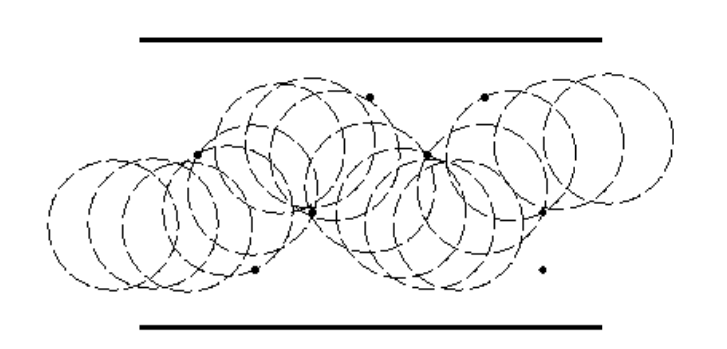
\includegraphics[width=0.5\textwidth]{img/fatman}
  \end{center}
  \ppage{Fatman Image from CPBook4 (Steven Halim)}

  One way to solve some problems is to break them down into smaller
  components.

  \begin{block}{}
  \begin{enumerate}
  \item Is it possible for a circle of radius $R, 0 \leq R \leq W$ to pass?
  \item What is the maximum $R$ that can pass?
  \end{enumerate}
  \end{block}

  \alert{QUIZ}: Assume that (1) is ``fast enough'', how do we solve (2)?
\end{frame}

\begin{frame}
  \frametitle{UVA 295 -- Fatman -- Binary Search}

    \begin{block}{}
      \begin{itemize}
      \item Is it possible for a circle of size $0 \leq R \leq W$ to pass?
      \item What is the maximum $R$ that can pass?
      \end{itemize}
    \end{block}

    If we have a "fast" function $T(R)$ that tests if $R$ can pass or not, we can use {\bf Binary Search} to find the maximum $R$ that pass:

    \bigskip

    \begin{enumerate}
    \item Start with $R_l = 0, R_h = W$, Test $T(R_l+R_h /2)$;
    \item If fails, $R_h = R_l+R_h/2$, else $R_l = (R_l+R_h)/2$; repeat $T(R_l+R_h/2)$.
    \item Repeat until $R_h - R_l < 0.0001$.
    \end{enumerate}

    This requires log$_2(100*10000) = 20$ operations.

    \bigskip

    \alert{QUIZ:} How can we test $T(R)$ ``fast enough''?
\end{frame}

\begin{frame}
  \frametitle{UVA 295 -- Fatman -- Squeezing through}

    \begin{center}
      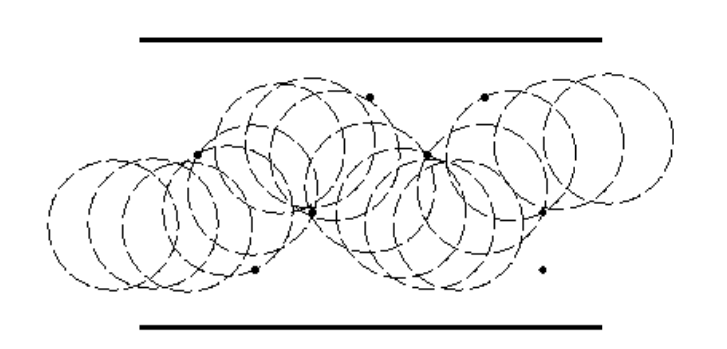
\includegraphics[width=0.4\textwidth]{img/fatman}
    \end{center}

    \begin{itemize}
    \item R can pass between two objects $i$ and $j$ if \emph{euclid}$(i,j) \geq R$
    \item R can pass between an object $i$ and a wall if $y_i \geq R || y_i \leq W-R$
    \end{itemize}

    \begin{exampleblock}{Algorithm for T(R)}
      \begin{itemize}
      \item Create a Graph $G$ where the obstacles and walls are vertices;
      \item If R can {\bf not} pass between $i$ and $j$, add an Edge $E_{ij}$;
      \item If there is a {\bf path} between both walls, \alert{R cannot pass};
      \end{itemize}
    \end{exampleblock}
\end{frame}

\begin{frame}[fragile]
  \frametitle{UVA 295 -- Fatman -- Squeezing through}

  {\smaller
  \begin{block}{T(R) sample code -- part 1, construct graph}
\begin{verbatim}
def test(R):
  nb = []                  # list of neighbor list
  for i in range(len(N)+2): nb[i] = list()

  for i in range(len(N)):  # N is list (x,y) of obstacles
    if (N[i][1] < R): nb[0].append(i+1)
    if (W - N[i][1] < R): nb[len(N)+1].append(i+1)
    if (i+1) in nb[0] and (i+1) in nb[len(N)+1]: return 0  # quick check 1
  if not (len(nb[0]) and len(nb[len(N)+1]): return 1       # quick check 2

  for i in range(len(N)):
    for j in range(len(N)):
      if dist(N[i],N[j]) < R: nb[i+1].append(j+1)
  ... next we test the graph ...
\end{verbatim}
  \end{block}
  }
\end{frame}


\begin{frame}[fragile]
  \frametitle{UVA 295 -- Fatman -- Squeezing through}


  {\smaller
    \alert{QUIZ:} What is the total cost of this approach?

    \begin{block}{T(R) sample code -- part 2, testing the graph}
\begin{verbatim}
def test(R):
  nb = []                  # list of neighbor list
  for i in range(len(N)+2): nb[i] = list()
  for i in range(len(N)):   ... border test ...
  for i in range(len(N)):
    for j in range(len(N)): ... build graph ...

  curnode = 0; visited = list(); tovisit = list()
  while 1: # DFS
    if (curnode == len(N)+1) return 0   # reached wall
    visited.add(curnode)
    for i in nb[curnode]: tovisit.append(i)
    while(curnode in visited):
       if not (len(tovisit)): return 1  # not reached wall
       curnode = tovisit.pop()
\end{verbatim}
    \end{block}
  }
\end{frame}

\subsection{Copying Books}
\begin{frame}[fragile]
  \frametitle{UVA 714 -- Copying books}

  {\smaller
    \begin{block}{Problem Description}
      \begin{itemize}
      \item There are $M$ books and $K$ scribes $(1 \leq K \leq M \leq 500)$.
      \item The each book has $p_i$ pages $(1 \leq p_i \leq 1000000)$
      \item Assign books to each scribe, and {\bf minimize} maximum job.
      \item Books must be assigned in blocks.
      \end{itemize}
    \end{block}

\begin{verbatim}
9 3
Input 1: 100 200 300 400 500 600 700 800 900
Output 1: 100 200 300 400 500 / 600 700 / 800 900 (max 1700)

5 4
Input 2: 100 100 100 100 100
Output 2: 100 / 100 / 100 / 100 100 (max 200)
\end{verbatim}

\begin{itemize}
\item \alert{QUIZ:} Describe the full search (and complexity)
\item \alert{QUIZ:} Describe a better algorithm?
\end{itemize}

  }
\end{frame}

\begin{frame}[fragile]
  \frametitle{UVA 714 -- Copying books -- Decomposition approach}

\begin{verbatim}
9 3
Input 1: 100 200 300 400 500 600 700 800 900
Output 1: 100 200 300 400 500 / 600 700 / 800 900 (max 1700)

5 4
Input 2: 100 100 100 100 100
Output 2: 100 / 100 / 100 / 100 100 (max 200)
\end{verbatim}

\vfill

    \begin{itemize}
    \item Someone has probably suggested DP. It is certainly possible.
    \item We could also use ``Binary Search + Test'' from the last problem:
      \begin{itemize}
      \item Binary search the maximum cost (100000*500 = 26 comparisons)
      \item Test if the maximum cost is possible (T(max))
      \item \alert{QUIZ:} What is a ``fast enough'' algorithm for T(max)?
      \end{itemize}
    \end{itemize}
\end{frame}

\begin{frame}[fragile]
  \frametitle{UVA 714 -- Copying books -- Testing a solution}
  {\smaller

\begin{verbatim}
9 3
Input 1: 100 200 300 400 500 600 700 800 900
Output 1: 100 200 300 400 500 / 600 700 / 800 900 (max 1700)
\end{verbatim}

\vfill

\begin{block}{One possible Test: Greedy Algorithm to test Maximum M}
\begin{verbatim}
def test(M):
  scribe = 0; book = 0;
  while scribe < K:
    sum = 0
    while sum + page[book] < M:
      sum += page[book]; book += 1
      if book == M: return 1   # assigned all books
    scribe ++
  return 0                     # did not assign all books
\end{verbatim}
\end{block}

  }
\end{frame}

\subsection{A careful Approach}
\begin{frame}[fragile]
  \frametitle{UVA 1079 -- A careful Approach}

  {\smaller
    \begin{block}{Problem Description}
      \begin{itemize}
      \item Choose the landing time $t_i$ for $2 \leq N \leq 8$ planes;
      \item The minimum gap $|t_i - t_j|$ must be as large as possible;
      \item Each plane $i$ has a maximum and minimum allowed landing time:\\
        $0 \leq \text{min}_i \leq t_i \leq \text{max}_i \leq 1440$
      \end{itemize}
    \end{block}

\begin{verbatim}
Input:               Solution:
3 planes             Maximum Minimum Gap: 7.5 minutes
1- 0 to 10           P1 - Arrive at 0
2- 5 to 15           P2 - Arrive at 7.5
3- 10 to 15          P3 - Arrive at 15
\end{verbatim}
  }

How do you solve it? (1- Binary search the GAP, 2- full search plane order, 3-greedy
for landing time)
\end{frame}

\begin{frame}

  \begin{center}
    The End -- Have a nice summer!
  \end{center}
\end{frame}
